\documentclass{article}
%\usepackage[utf8]{inputenc}
\usepackage{geometry}
%\usepackage{polski}
\usepackage{float}
\usepackage{graphicx}
\usepackage[shortlabels]{enumitem}
\usepackage{amsmath}
\usepackage{amsthm}
\usepackage{amsfonts}
\usepackage{amssymb}
\usepackage{hyperref}
\usepackage{array}

\usepackage{xcolor}
\usepackage{indentfirst}
\usepackage{caption}
\usepackage{subcaption}




\title{Report 2}
\author{Aleksander Jakóbczyk and Bogdan Banasiak\\ 
	Index number: 255939 and 256456}
\date{}\date{}

\newtheorem{theorem}{Theorem}
\newtheorem{definition}{Definition}

\DeclareMathOperator{\sign}{sign}
\renewcommand{\thesubsubsection}{\thesubsection. \roman{subsubsection})}
\setcounter{section}{-1}

\makeatletter
\newif\if@mathitemize
\newif\if@closemathitem
\let\orig@item=\item
\renewcommand{\item}{\if@closemathitem$\fi\orig@item\if@mathitemize\@closemathitemtrue$\fi}
\newenvironment{mathitemize}{\@mathitemizetrue\itemize\@closemathitemfalse}{$\enditemize}
\makeatother

\begin{document}
	\maketitle
	\section{Information and formulas}
	
	
	\subsection{Discrete alpha-stable vector}
	In case when $\Gamma$ is a discrete spectral measure with a finite number of point masses, i.e.,
	\begin{equation}\label{Discrete spectral measure}
		\Gamma(\cdot)=\sum_{j=1}^n \gamma_j \delta_{\mathbf{s}_j}(\cdot),
	\end{equation}
	where $\gamma_j$ are the weights, and $\delta_{\mathbf{s}_j}$ are point masses at the points $\mathbf{s}_j \in S_d, j=1,2 \ldots, n$. \\$\left(S_d=\left\{\mathbf{x} \in \mathbb{R}^d:\|x\|=1\right\}\right)$.
	For such discrete spectral measure \eqref{Discrete spectral measure}, the characteristic function of $\mathbf{X} \sim S_{\alpha, d}\left(\Gamma, \mu^0=\mathbf{0}\right)$
	\begin{equation*}
		\mathbb{E} \exp \{i\langle\mathbf{X}, \mathbf{t}\rangle\},
	\end{equation*}

	takes the form
	\begin{equation}\label{Discrete cf}
		\phi^*(\mathbf{t})=\exp \left(-\sum_{j=1}^n \psi_\alpha\left(\left\langle\mathbf{t}, \mathbf{s}_j\right\rangle\right) \gamma_j\right),
	\end{equation}
	where $\psi_\alpha$ is given by
	$$
	\psi_\alpha(u)= \begin{cases}|u|^\alpha(1-i \operatorname{sign}(u)) \tan \frac{\pi \alpha}{2}, & \alpha \neq 1, \\ |u|\left(1+i \frac{2}{\pi} \operatorname{sign}(u)\right) \log |u|, & \alpha=1 .\end{cases}
	$$
	Following result from Modarres and Nolan, if $\mathbf{X}$ has a characteristic function \eqref{Discrete cf}, then
	$$
	\mathbf{X} \stackrel{D}{=} \begin{cases}\sum_{j=1}^n \gamma_j^{1 / \alpha} Z_j \mathbf{s}_j, & \alpha \neq 1, \\ \sum_{j=1}^n \gamma_j^{1 / \alpha}\left(Z_j+\frac{2}{\pi} \log \gamma_j\right) \mathbf{s}_j, & \alpha=1,\end{cases}
	$$
	where $Z_1, Z_2, \ldots, Z_n$ are i.i.d. totally skewed, standardized one dimensional $\alpha$-stable random variables, i.e. $Z_i \sim S_\alpha\left(\beta=1, \gamma=1, \delta=0\right.$ ). (When $\mu^{\mathbf{0}} \neq \mathbf{0}$, both cases above have a $+\mu^{\mathbf{0}}$ in them.)
	
	\subsection{Stable vector}
	The characteristic function of $\mathbf{X} \sim S_{\alpha, d}\left(\Gamma, \mu^0\right)$ is
	$$
	\phi_{\mathbf{X}}(\mathbf{t})=\mathbf{E} \exp \{i<\mathbf{X}, \mathbf{t}>\}=\exp \left(-I_{\mathbf{X}}(\mathbf{t})+i<\mu^0, t>\right),
	$$
	where the function in the exponent is
	$$
	I_{\mathbf{X}}(\mathbf{t})=\int_{S_d} \psi_\alpha(<\mathbf{t}, \mathbf{s}>) \Gamma(d s) .
	$$
	Here $<\mathbf{t}, \mathbf{s}>=t_1 s_1+\cdots+t_d s_d$ is the inner product, and
	$$
	\psi_\alpha(u)= \begin{cases}|u|^\alpha\left(1-i \operatorname{sign}(u) \tan \frac{\pi \alpha}{2}\right) & \alpha \neq 1, \\ 
		|u|\left(1+i \frac{2}{\pi} \operatorname{sign}(u) \ln |u|\right) & \alpha=1.\end{cases}
	$$
	
	\subsection{Sub-Gaussian vectors}\label{formula1}
	Choose a random variable $A \sim S_{\alpha / 2}\left(\gamma=\left(\cos \frac{\pi \alpha}{4}\right)^{2 / \alpha}, \beta=1, \delta=0\right)$ with $\alpha<2$. Let $\mathbf{G}=\left[G_1, G_2, \ldots, G_d\right]$ be a zero mean Gaussian vector in $\mathbb{R}^d$ independent of $A$. Then the random vector
	\begin{equation}
		\mathbf{X}=\left[A^{1 / 2} G_1, A^{1 / 2} G_2, \ldots, A^{1 / 2} G_d\right],
	\end{equation}

	has symmetric $\alpha$-stable distribution in $\mathbb{R}^d$ and is called a sub-Gaussian SaS random vector in $\mathbb{R}^d$ with underlying Gaussian vector $\mathbf{G}$.
	Your goal is to check if the following statements, assuming the underlying Gaussian vector $\mathbf{G}$ has i.i.d. components with variance $\sigma^2$.
	
	\subsection{Estimation of spectral measure}
	We use the Rachev-Xin-Cheng method (RXC). A value is picked for $r$ and it is used to estimate the measure of as set $A \subset S_d$ by
	$$
	\widehat{\Gamma}(A)=\text { const. } \frac{\#\left\{\mathbf{X}_i:\left|\mathbf{X}_i\right|>r, \mathbf{X}_i \in \operatorname{Cone}(A)\right\}}{\#\left\{\mathbf{X}_i:\left|\mathbf{X}_i\right|>r\right\}} .
	$$
	
	\subsection{Estimation of characteristic function} \label{teoCF}
	The empirical characteristic function (ECF) method is straightforward. Given an i.i.d. sample $\mathbf{X}_1, \ldots, \mathbf{X}_k$ of $\alpha$-stable random vectors with spectral measure $\Gamma$, let $\widehat{\varphi}_k(\mathbf{t})$ and $\widehat{I}_k$ be the empirical counterparts of $\phi$ and $I$, i.e. $\widehat{\varphi}_k(\mathbf{t})=(1 / k) \sum_{j=1}^k \exp \left(i<\mathbf{t}, \mathbf{X}_j>\right)$ is the sample characteristic function, and $\widehat{I}_k(\mathbf{t})=-\ln \widehat{\varphi}_k(\mathbf{t})$. Given a grid $\mathbf{t}_1, \ldots, \mathbf{t}_n \in S_d, \vec{I}_{E C F, k}=\left[\hat{I}_k\left(\mathbf{t}_1\right), \ldots, \hat{I}_k\left(\mathbf{t}_n\right)\right]^{\prime}$ is the ECF estimate of $I_{\mathbf{X}}(\cdot)$.
	
	\subsection{Codifference estimator}
	Let us define the codiffence between random variables $X$ and $Y$ in the following way:
	\begin{equation}
		\tau_{X, Y}=\log (\mathbb{E} \exp (i(X-Y)))-\log (\mathbb{E} \exp (i X))-\log (\mathbb{E} \exp (-i Y)).
	\end{equation}

	\section{Multivariate stable distribution generator}
	
	We checked if our generator was implemented correctly, by generating 20000 of two-dim vectors
	
	\subsection{Symmetric stable vector}
	For following parameters, we generated vectors and we created plot~\ref{1} - dependence of x and y obtained in vectors.
	Symmetric case $\alpha=0.9$ and $n=6$ point masses
	\begin{mathitemize}
		\item \gamma_1  =0.25 \text { at } \mathbf{s}_1=(1,0) ,
		\item \gamma_2  =0.125 \text { at } \mathbf{s}_2=(1 / 2, \sqrt{3} / 2) ,
		\item \gamma_3  =0.25 \text { at } \mathbf{s}_3=(-1 / 2, \sqrt{3} / 2) ,
		\item \gamma_4  =0.25 \text { at } \mathbf{s}_4=(-1,0) ,
		\item \gamma_5  =0.125 \text { at } \mathbf{s}_5=(-1 / 2,-\sqrt{3} / 2),
		\item \gamma_6  =0.25 \text { at } \mathbf{s}_6=(1 / 2,-\sqrt{3} / 2).
	\end{mathitemize}
	
	\begin{figure}[H]
		\centering
		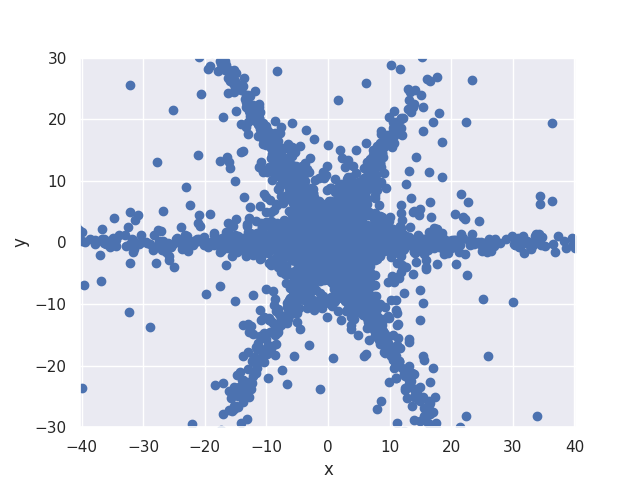
\includegraphics[width=1\linewidth]{images/ex_1_a_alpha_stable_vector_simulation_symmetric_discreet_scatter.png}
		\caption{Result of simulation of symmetric stable vector for $\alpha=0.9$ and $n=6$.}\label{1}
	\end{figure}
	
	We can observe that points are located on six different direction lines, so we can conclude, that the implementation of our generator in this case should be correct.
	
	\subsection{Stable vector with independent components}
	
	In this case, we generated vectors using formula from \ref{formula1}. 
	We used the following covariance matrix 
	\begin{equation*}
		\Sigma(G) = \left[{\begin{array}{*{20}c}
			1 & 0\\
			0 & 1\end{array} } \right].
	\end{equation*}
	
	By using a covariance matrix with zeros on anti-diagonal, we obtain i.i.d. vectors A and G and elements of generated Gaussian vector are independent.
	
	We are checking the correctness of the simulation in section 2.
	
	\begin{figure}[H]
		\centering
		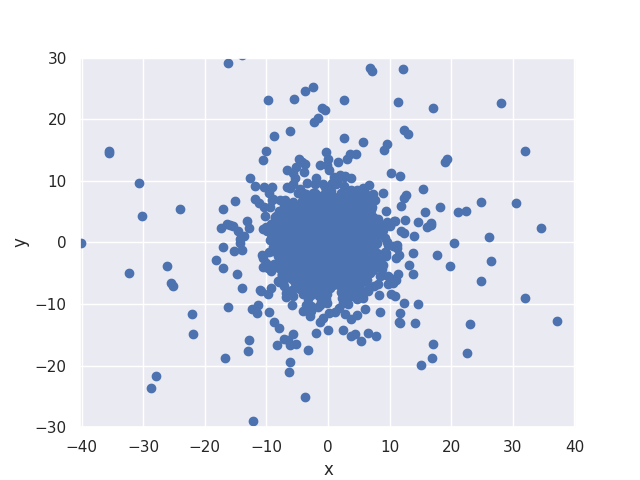
\includegraphics[width=1\linewidth]{images/ex_1_b_alpha_stable_vector_simulation_symmetric_continous_scatter}
		\caption{Result of stable vector with independent components for $\alpha=1.6$.}\label{2}
	\end{figure}
	Thanks to the results we obtained and are depicted on graph \ref{2}, we can conclude, that in this case, vectors are also simulated correctly.
	
	\subsection{Stable vector which is not symmetric and has not independent components.}
	
	In this case, matrix of covariance is equal
	\begin{equation*}
		\Sigma(G) = \left[{\begin{array}{*{20}c}
			1 & 0.5\\
			0.5 & 0.7\end{array} } \right],
	\end{equation*}

	so, the covariance of vector G is not zero and elements of this vector are not independent. It means that vector components of vector X are not independent. What's more, in vector G, the variance of the first element is different from the second one, so generated vectors are not symmetric.
	
	\begin{figure}[H]
		\centering
		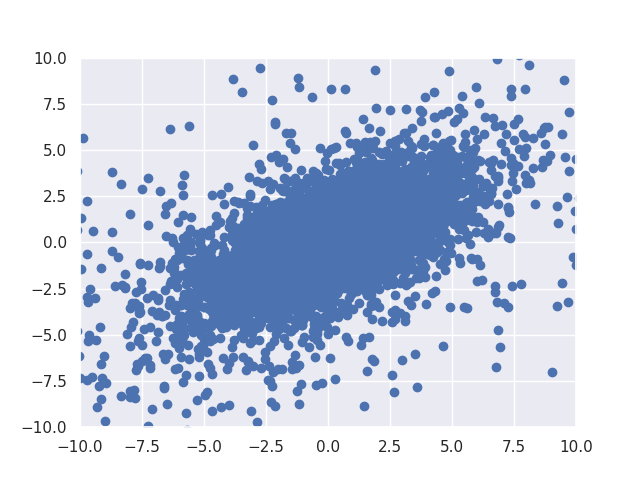
\includegraphics[width=1\linewidth]{images/ex_1_c_alpha_stable_vector_simulation_symmetric_discreet_scatter}
		\caption{Result of $\alpha$ stable vector which is not symmetric and has not independent components for $\alpha=1.6$.}\label{3}
	\end{figure}
	The results, shown on the graph \ref{3} confirm the theoretical assumptions, so we can assume that our implementation works correctly in this case as well.
	
	\section{Sub-Gaussian random vector generator.}\label{sec2}
	
	To check if our implementation of sub-Gaussian random vector generator, we generated 20000 of random vectors using the method described in subsection \ref{formula1}, where $\alpha = 1.6$ and the following covariance matrix:
	\begin{equation*}
		\Sigma(G) = \left[{\begin{array}{*{20}c}
			1 & 0\\
			0 & 1\end{array} } \right].
	\end{equation*}
	
	\begin{figure}\label{dwa}
		\centering
		\begin{subfigure}[H]{0.49\textwidth}
			\centering
			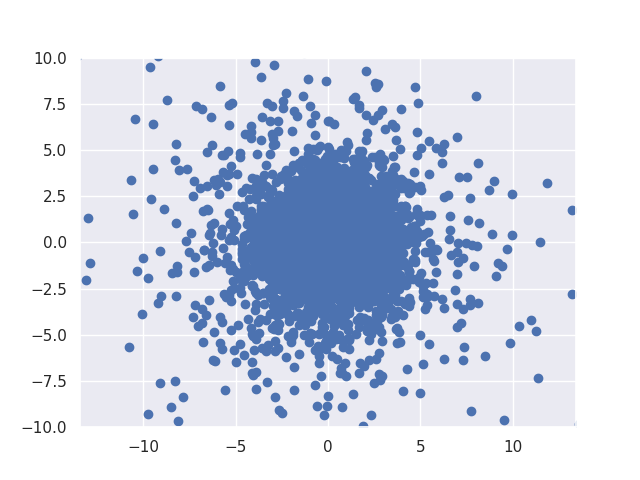
\includegraphics[width=\textwidth]{images/ex_2_alpha_stable_vector_simulation_sub_gaussian_SaS_catter}
			\caption{Generated sub-Gaussian random vectors.}\label{4}
		\end{subfigure}
		\hfill
		\begin{subfigure}[H]{0.49\textwidth}
			\centering
			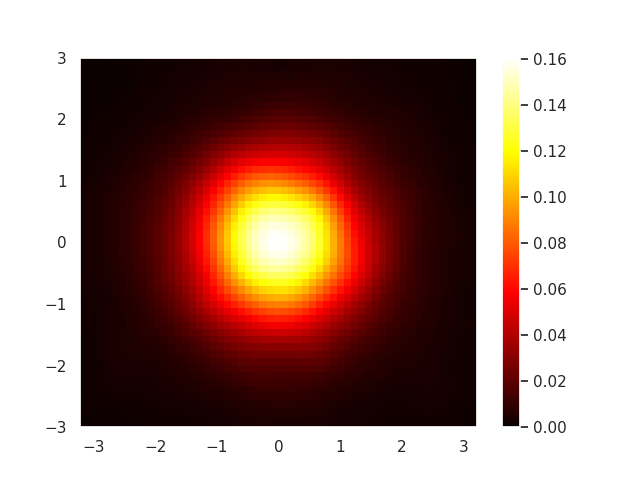
\includegraphics[width=\textwidth]{images/ex_2_alpha_stable_vector_simulation_sub_gaussian_SaS_heatmap}
			\caption{Two-dimensional density of generated vectors.}\label{5}
		\end{subfigure}
		\caption{Result of simulation of Sub-Gaussian random vector for $\alpha = 1.6$.}
	\end{figure}
	
	At the graph \ref{4} we presented the dependence of first and second values of generated vectors. In addition, on graph \ref{5}, we presented empirical two-dimensional density of the scatter plot. We can see that the results are symmetric. 
	
	\begin{figure}[H]
		\centering
		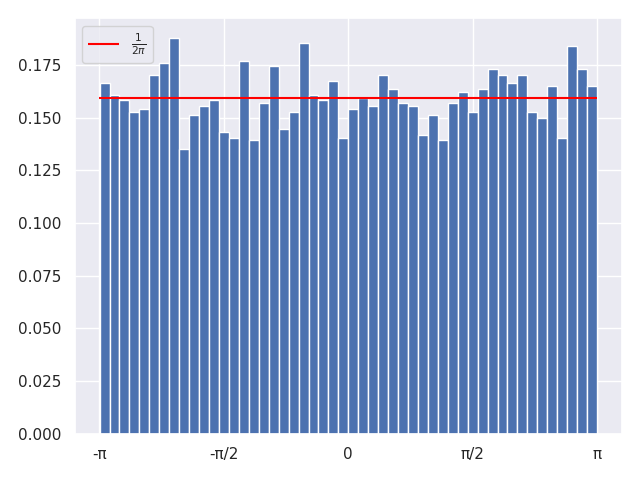
\includegraphics[width=0.8\linewidth]{images/ex_2_spectral_measure}
		\caption{Estimated spectral measure.}\label{6}
	\end{figure}
	
	We also checked spectral measure, the results are depicted at the graph \ref{5}, where a horizontal red line is equal to $\frac{1}{2 \pi}$ what is the value of density of uniform distribution from $-\pi$ to $\pi$. 
	We also checked, using KS-test, if results are uniformly distributed. We got p-value = $0.96$ , so based on the graph and the result of the KS-test, we can conclude, that the spectral measure is uniformly distributed.
	
	We estimated CF of S$\alpha$S random vector, which is presented at graph \ref{7} and at graph \ref{8} we have included errors between the estimated and the theoretical function. Additionally, in table \ref{tab1}, we included basic statistics of these errors. We can observe that errors are really small.
	
	\begin{figure}
		\centering
		\begin{subfigure}[H]{0.49\textwidth}
			\centering
			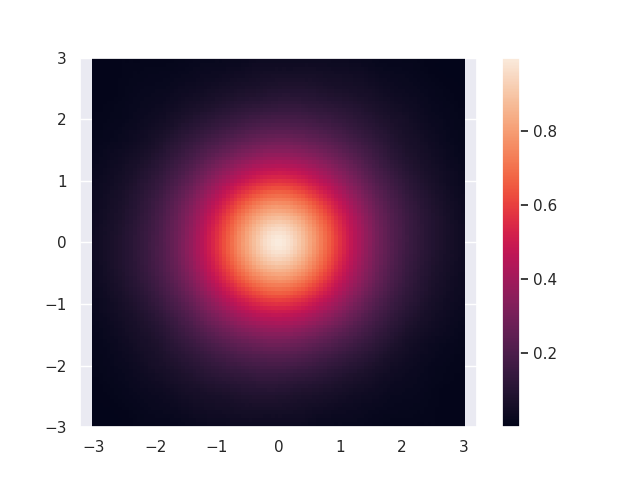
\includegraphics[width=1\linewidth]{images/ex_2_ecf}
			\caption{ECF of generated vectors.}\label{7}
		\end{subfigure}
		\hfill
		\begin{subfigure}[H]{0.49\textwidth}
			\centering
			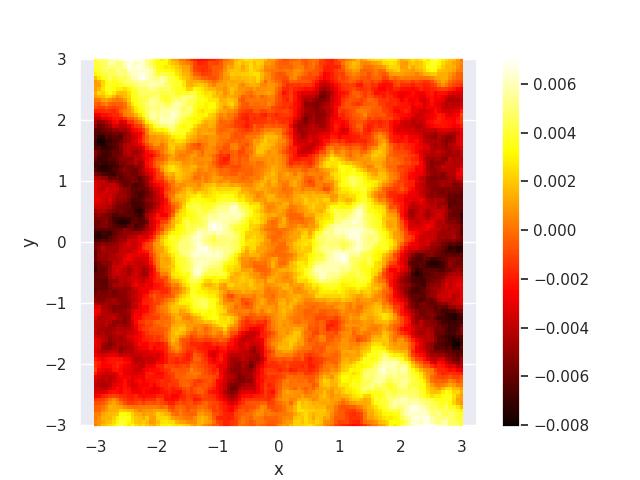
\includegraphics[width=1\linewidth]{images/ex_2_error_heatmap}
			\caption{Errors of comparison of theoretical and empirical CF of SaS random vector.}\label{8}
		\end{subfigure}
		\caption{Result of estimate characteristic function for sub-Gaussian stable vector for $\alpha = 1.6$.}
	\end{figure}
	
	\begin{table}[H]
		\centering
		\begin{tabular}{rrrrrrrr}
			\hline
			count &      mean &      std &      min &       25\% &       50\% &       75\% &       max \\
			\hline
			10000.0 & -0.000252 &  0.00322 & -0.00809 & -0.002605 & -0.000049 &  0.001813 &  0.007082 \\
			\hline
		\end{tabular}
		\caption{Basic statistics of errors between the estimated and the theoretical characteristic function.}\label{tab1}
	\end{table}
	
	
	\section{Estimation of \texorpdfstring{$\alpha$ } and spectral measure \texorpdfstring{$\Gamma$}.}
	
	Using the method described in \ref{teoCF}, we were able to fit the correct function to double-logarithm characteristic function and based on knowledge of CF from section 4 we estimated parameter $\alpha$.
	
	\begin{figure}[H]
		\centering
		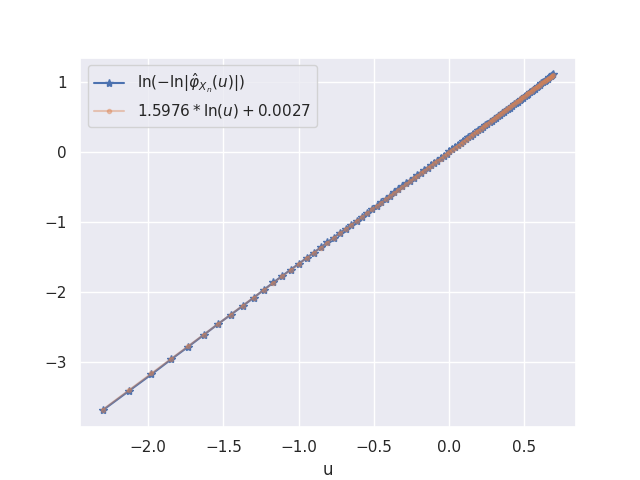
\includegraphics[width=0.8\linewidth]{images/compare_cf}
		\caption{Fitted function to empirical double-logarithm CF.}\label{11}
	\end{figure}
	In this case we used the same parameters as in section \ref{sec2}. We estimated $\alpha$ 1000 times using samples with size of 10000.
	
	We created two graphs (\ref{9}, \ref{10}), histogram and boxplot of estimated parameter $\alpha$.
	
	\begin{figure}
		\centering
		\begin{subfigure}[H]{0.49\textwidth}
			\centering
			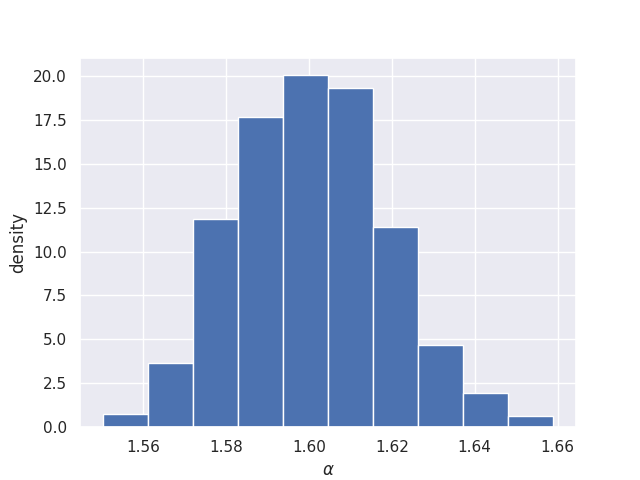
\includegraphics[width=1\linewidth]{images/cf_alpha_estimation_hist}
			\caption{Histogram of estimated $\alpha$.}\label{9}
		\end{subfigure}
		\hfill
		\begin{subfigure}[H]{0.49\textwidth}
			\centering
			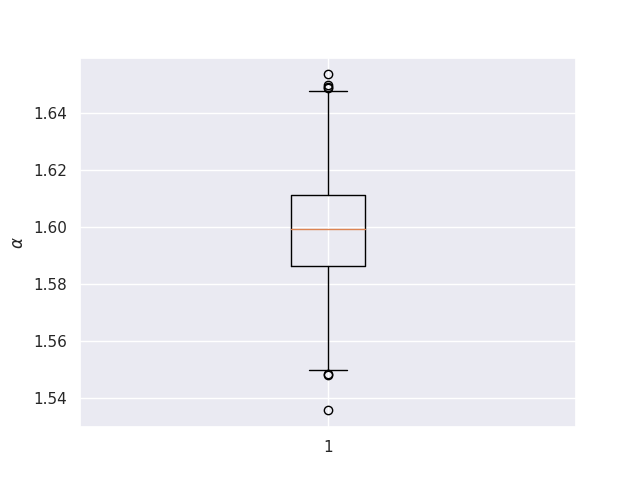
\includegraphics[width=1\linewidth]{images/cf_alpha_estimation_boxplot}
			\caption{Boxplot of estimated $\alpha$.}\label{10}
		\end{subfigure}\caption{Estimation's results of $\alpha$.}
	\end{figure}
	
	Basic statistics of our estimations we have located in table \ref{tab2}
	
	\begin{table}[H]
		\centering
		\begin{tabular}{rrrrrrrr}
			\hline
			count &      mean &      std &       min &       25\% &       50\% &       75\% &      max \\
			\hline
			1000.0 &  1.599539 &  0.01839 &  1.535825 &  1.586632 &  1.599462 &  1.611326 &  1.65366 \\
			\hline
		\end{tabular}
		\caption{Basic statistics of estimated $\alpha$.}\label{tab2}
	\end{table}
	
	We can see that the mean is close to true $\alpha$ and variance is low. We also obtained a small range.
	
	\section{Estimation of the characteristic function for multivariate data}
	Using the method described in \ref{teoCF} by function $I(x)$ We can estimate CF for a stable vector.
	As an example, we estimated CF for vectors with the same parameters as in section \ref{sec2}. (Graph \ref{12})
	\begin{figure}[H]
		\centering
		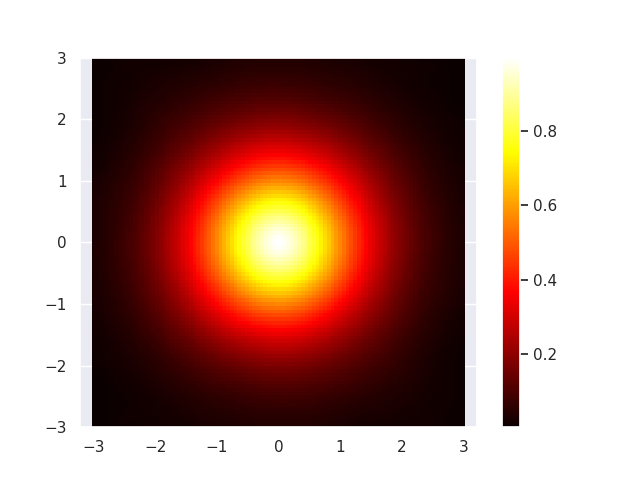
\includegraphics[width=1\linewidth]{images/ex_4_cf_sub_gaussian_SaS}
		\caption{Characteristic function of sub-gaussian.}\label{12}
	\end{figure}
	
	\section{Estimation of codifference measure}
	To check the correctness of our estimator implementation, we have generated 100000 samples thanks to which we estimated codifference for particular cases.
	
	\subsection{First case}
	Parameters:
	\begin{mathitemize}
		\item \alpha    =1.6 ,
		\item \gamma_1 =0.25 \text{ at } \mathbf{s}_1=(1,0),
		\item \gamma_2 =0.25 \text{ at } \mathbf{s}_2=(0,1),
		\item \gamma_3 =0.25 \text{ at } \mathbf{s}_3=(-1,0),
		\item \gamma_4 =0.25 \text{ at } \mathbf{s}_4=(0,-1).
	\end{mathitemize}
	
	\begin{figure}[H]
		\centering
		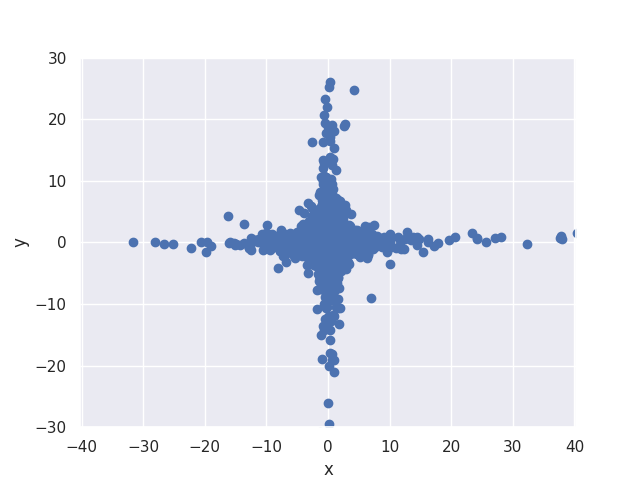
\includegraphics[width=1\linewidth]{images/ex_5_1_alpha_stable_vector_simulation_discreet_scatter}
		\caption{Result of simulation.}\label{13}
	\end{figure}
	
	Codifference = 0.0158.
	
	\subsection{Second case}
	Parameters:
	\begin{mathitemize}
		\item \alpha   =0.9 ,
		\item \gamma_1 =0.25 \text {at } \mathbf{s}_1=(\sqrt{2} / 2, \sqrt{2} / 2),
		\item \gamma_2 =0.25 \text{ at } \mathbf{s}_2=(-\sqrt{2} / 2, \sqrt{2} / 2),
		\item \gamma_3 =0.25 \text{ at } \mathbf{s}_3=(-\sqrt{2} / 2,-\sqrt{2} / 2),
		\item \gamma_4 =0.25 \text{ at } \mathbf{s}_4=(\sqrt{2} / 2,-\sqrt{2} / 2).
	\end{mathitemize}
	
	\begin{figure}[H]
		\centering
		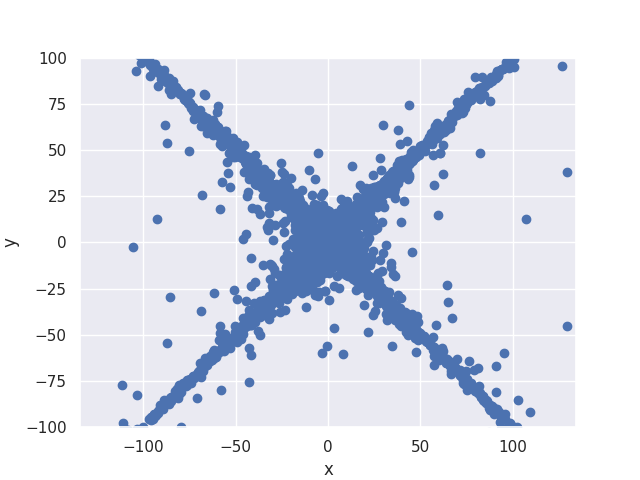
\includegraphics[width=1\linewidth]{images/ex_5_2_alpha_stable_vector_simulation_discreet_scatter}
		\caption{Result of simulation.}\label{14}
	\end{figure}
	
	Codifference = 0.7933.
	
	\subsection{Third case}
	Sub-Gaussian vector with $\alpha =1.6$ covariance matrix
	\begin{equation*}
		\Sigma(G) = \left[{\begin{array}{*{20}c}
			1 & 0.5\\
			0.5 & 1\end{array} } \right].
	\end{equation*}
	
	\begin{figure}[H]
		\centering
		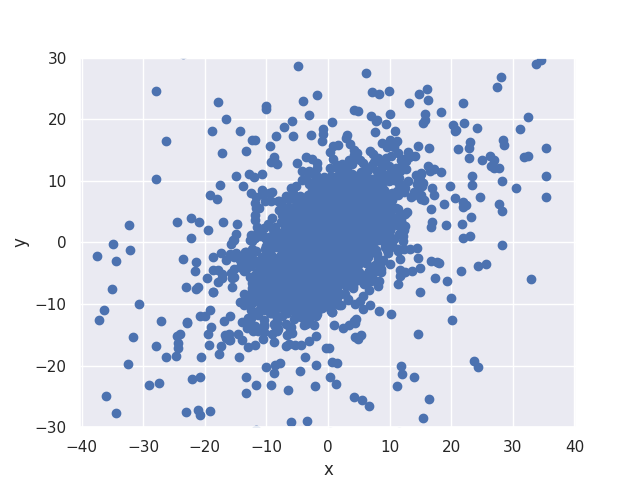
\includegraphics[width=1\linewidth]{images/ex_5_3_alpha_stable_vector_simulation_continuous_scatter}
		\caption{Result of simulation.}\label{15}
	\end{figure}
	
	Codifference = 0.5778.
	
	
	
	\section{Summary}
	We checked correctness of implementation of all methods and estimators. In every case, we obtained good results.
	
\end{document}
